%email an gerhard.kniewasser@student.tugraz.at

% **************************************************************************************************
% ** SPSC Report and Thesis Template
% **************************************************************************************************
%
% ***** Authors *****
% Daniel Arnitz, Paul Meissner, Stefan Petrik
% Signal Processing and Speech Communication Laboratory (SPSC)
% Graz University of Technology (TU Graz), Austria
%
% ***** Changelog *****
% 0.1   2010-01-25   extracted from report template by Daniel Arnitz (not ready yet)
% 0.2   2010-02-08   added thesis titlepage and modified layout (not ready yet)
% 0.3   2010-02-18   added TUG logo and statutory declaration
% 0.4   2010-02-18   moved the information fields below % **************************************************************************************************
% ** SPSC Report and Thesis Template
% **************************************************************************************************
%
% ***** Authors *****
% Daniel Arnitz, Paul Meissner, Stefan Petrik
% Signal Processing and Speech Communication Laboratory (SPSC)
% Graz University of Technology (TU Graz), Austria
%
% ***** Changelog *****
%
% ***** Todo *****
%
% **************************************************************************************************



\documentclass[%
a4paper,% !!! ATTENTION: geometry package below !!!
\Twosided,% !!! ATTENTION: geometry package below !!!
openany,% begin chapters with new right page (openright) or don't care (openany)
11pt,%
fleqn,% equations not centered, but on the left side
tablecaptionbelow,% captions below tables
% titlepage,% use title
pointlessnumbers,% do not generate point at the end of section numbers (e.g. 1.4.5 instead of 1.4.5.)
final,%
]{scrreprt}% (KOMA)

\usepackage[paper=a4paper,\Twosided,%
textheight=246mm,%
textwidth=160mm,%
heightrounded=true,% round textheight to multiple of lines (avoids overfull vboxes)
ignoreall=true,% do not include header, footer, and margins in calculations
marginparsep=5pt,% marginpar only used for signs (centered), thus only small sep. needed
marginparwidth=10mm,% prevent margin notes to be out of page
hmarginratio=2:1,% set margin ration (inner:outer for twoside) - (2:3 is default)
]{geometry}%


% master
\usepackage{ifthen}% for optional parts
\usepackage[utf8]{inputenc}% German special characters
\ifthenelse{\equal{\DocumentLanguage}{en}}{\usepackage[USenglish]{babel}}{}%
\ifthenelse{\equal{\DocumentLanguage}{de}}{\usepackage[ngerman]{babel}}{}%
\usepackage[%
headtopline,plainheadtopline,% activate all lines (header and footer)
headsepline,plainheadsepline,%
footsepline,plainfootsepline,%
footbotline,plainfootbotline,%
automark% auto update \..mark
]{scrpage2}% (KOMA)
\usepackage{makeidx}% used to make an index directory
\usepackage[]{caption}% customize captions
\usepackage{multicol}%
\usepackage[stable,bottom,hang,splitrule,multiple,symbol*]{footmisc}% customize footnotes


% text
\usepackage{varioref}% improved references
\usepackage{color}% e.g., for color boxes
\usepackage{rotating}% to rotate objects
\usepackage{gensymb}% symbols (perthousand, Celsius, ...)
\usepackage[right]{eurosym}% euro symbol on the right side (51 EUR)
\usepackage[normalem]{ulem}% cross-out, strike-out, underlines (normalem: keep \emph italic)
%\usepackage[safe]{textcomp}% loading in safe mode to avoid problems (see LaTeX companion)
%\usepackage[geometry,misc]{ifsym}% technical symbols
\usepackage{remreset}%\@removefromreset commands (e.g., for continuous footnote numbering)
\usepackage[%
breaklinks=true,% allow line break in links
colorlinks=true,% if false: framed link
linkcolor=black,anchorcolor=black,citecolor=black,filecolor=black,%
menucolor=black,urlcolor=black]{hyperref}% hyperlinks for references


% math
\usepackage{amsmath,amssymb,amstext,bm} % use math packages
\usepackage{mathcomp}% symbols (perthousand, ...) in math mode


% graphics
\usepackage{graphicx}% use simple graphics
\usepackage{subfigure}% subfigures (a),(b),(c)... within figures
\usepackage{flafter}% place floats always after reference
\usepackage{placeins}% preventing floats from crossing a barrier
\usepackage{float}% to place floats !HERE!
\usepackage{psfrag}% replace text in eps figures


% tables
\usepackage{hhline}% hline doesn't work with colored columns, so using hhline
\usepackage{longtable}% for tables longer than one page
\usepackage{dcolumn}% for number alignment in tables
\usepackage{colortbl}% color in tables


% listings
%\usepackage{alltt}% verbatim environment with commands available
\usepackage{listings}% program code listings


% other
%\usepackage{layout}% graphical page layout (spacings)
\usepackage{xspace}% add space after macros if not followed by punctuation character
\makeindex% used for index creation

 (encoding...)
% 0.5   2010-03-02   added \ShortTitle to fix problems with long thesis titles
%                    added \ThesisType (makes the template suitable for MSc, BSc, PhD, ... Thesis)
%
% ***** Todo *****
% - Introduction/Usage
% **************************************************************************************************

% **************************************************************************************************
% basic setup
\newcommand{\DocumentType}{report} % "thesis" / "report"
\newcommand{\DocumentLanguage}{de} % "en" / "de"
\newcommand{\Twosided}{} % "twoside" / ""


% **************************************************************************************************
% template setup -- do not change these unless you know what you are doing!
% **************************************************************************************************
% ** SPSC Report and Thesis Template
% **************************************************************************************************
%
% ***** Authors *****
% Daniel Arnitz, Paul Meissner, Stefan Petrik
% Signal Processing and Speech Communication Laboratory (SPSC)
% Graz University of Technology (TU Graz), Austria
%
% ***** Changelog *****
%
% ***** Todo *****
%
% **************************************************************************************************



\documentclass[%
a4paper,% !!! ATTENTION: geometry package below !!!
\Twosided,% !!! ATTENTION: geometry package below !!!
openany,% begin chapters with new right page (openright) or don't care (openany)
11pt,%
fleqn,% equations not centered, but on the left side
tablecaptionbelow,% captions below tables
% titlepage,% use title
pointlessnumbers,% do not generate point at the end of section numbers (e.g. 1.4.5 instead of 1.4.5.)
final,%
]{scrreprt}% (KOMA)

\usepackage[paper=a4paper,\Twosided,%
textheight=246mm,%
textwidth=160mm,%
heightrounded=true,% round textheight to multiple of lines (avoids overfull vboxes)
ignoreall=true,% do not include header, footer, and margins in calculations
marginparsep=5pt,% marginpar only used for signs (centered), thus only small sep. needed
marginparwidth=10mm,% prevent margin notes to be out of page
hmarginratio=2:1,% set margin ration (inner:outer for twoside) - (2:3 is default)
]{geometry}%


% master
\usepackage{ifthen}% for optional parts
\usepackage[utf8]{inputenc}% German special characters
\ifthenelse{\equal{\DocumentLanguage}{en}}{\usepackage[USenglish]{babel}}{}%
\ifthenelse{\equal{\DocumentLanguage}{de}}{\usepackage[ngerman]{babel}}{}%
\usepackage[%
headtopline,plainheadtopline,% activate all lines (header and footer)
headsepline,plainheadsepline,%
footsepline,plainfootsepline,%
footbotline,plainfootbotline,%
automark% auto update \..mark
]{scrpage2}% (KOMA)
\usepackage{makeidx}% used to make an index directory
\usepackage[]{caption}% customize captions
\usepackage{multicol}%
\usepackage[stable,bottom,hang,splitrule,multiple,symbol*]{footmisc}% customize footnotes


% text
\usepackage{varioref}% improved references
\usepackage{color}% e.g., for color boxes
\usepackage{rotating}% to rotate objects
\usepackage{gensymb}% symbols (perthousand, Celsius, ...)
\usepackage[right]{eurosym}% euro symbol on the right side (51 EUR)
\usepackage[normalem]{ulem}% cross-out, strike-out, underlines (normalem: keep \emph italic)
%\usepackage[safe]{textcomp}% loading in safe mode to avoid problems (see LaTeX companion)
%\usepackage[geometry,misc]{ifsym}% technical symbols
\usepackage{remreset}%\@removefromreset commands (e.g., for continuous footnote numbering)
\usepackage[%
breaklinks=true,% allow line break in links
colorlinks=true,% if false: framed link
linkcolor=black,anchorcolor=black,citecolor=black,filecolor=black,%
menucolor=black,urlcolor=black]{hyperref}% hyperlinks for references


% math
\usepackage{amsmath,amssymb,amstext,bm} % use math packages
\usepackage{mathcomp}% symbols (perthousand, ...) in math mode


% graphics
\usepackage{graphicx}% use simple graphics
\usepackage{subfigure}% subfigures (a),(b),(c)... within figures
\usepackage{flafter}% place floats always after reference
\usepackage{placeins}% preventing floats from crossing a barrier
\usepackage{float}% to place floats !HERE!
\usepackage{psfrag}% replace text in eps figures


% tables
\usepackage{hhline}% hline doesn't work with colored columns, so using hhline
\usepackage{longtable}% for tables longer than one page
\usepackage{dcolumn}% for number alignment in tables
\usepackage{colortbl}% color in tables


% listings
%\usepackage{alltt}% verbatim environment with commands available
\usepackage{listings}% program code listings


% other
%\usepackage{layout}% graphical page layout (spacings)
\usepackage{xspace}% add space after macros if not followed by punctuation character
\makeindex% used for index creation


\input{./base/layout_\DocumentType}
% **************************************************************************************************
% ** SPSC Report and Thesis Template
% **************************************************************************************************
%
% ***** Authors *****
% Daniel Arnitz, Paul Meissner, Stefan Petrik
% Signal Processing and Speech Communication Laboratory (SPSC)
% Graz University of Technology (TU Graz), Austria
%
% ***** Changelog *****
%
% ***** Todo *****
%
% **************************************************************************************************



% **************************************************************************************************
% * SECTIONING AND TEXT
% **************************************************************************************************

% new chapter, section, ... plus a few addons
%   part
\newcommand{\newpart}[2]{\FloatBarrier\cleardoublepage\part{#1}\label{part:#2}}%
%   chapter
\newcommand{\newchapter}[2]{\FloatBarrier\chapter{#1}\label{chp:#2}}
\newcommand{\newchapterNoTOC}[2]{\FloatBarrier\stepcounter{chapter}\chapter*{#1}\label{chp:#2}}%
%   section
\newcommand{\newsection}[2]{\FloatBarrier\vspace{5mm}\section{#1}\label{sec:#2}}%
\newcommand{\newsectionNoTOC}[2]{\FloatBarrier\vspace{5mm}\stepcounter{section}\section*{#1}\label{sec:#2}}%
%   subsection
\newcommand{\newsubsection}[2]{\FloatBarrier\vspace{3mm}\subsection{#1}\label{sec:#2}}%
\newcommand{\newsubsectionNoTOC}[2]{\FloatBarrier\vspace{3mm}\stepcounter{subsection}\subsection*{#1}\label{sec:#2}}%
%   subsubsection
\newcommand{\newsubsubsection}[2]{\vspace{2mm}\subsubsection{#1}\label{sec:#2}}%
\newcommand{\newsubsubsectionNoTOC}[2]{\vspace{2mm}\stepcounter{subsubsection}\subsubsection*{#1}\label{sec:#2}}%

% next paragraph
\newcommand{\nxtpar}{\par\bigskip}

% "stylish" quotes on the right side
\newcommand{\openingquote}[2]{\hfill\parbox[t]{10cm}{\itshape\raggedleft{"#1"}\\\footnotesize -- #2}\nxtpar}%

% direct quotes
% \newenvironment{directquote}{\nxtpar\hrule}{\hrule}\hfill\litref{#1}{#2}}

% warnings and attention signs in marginpar
\newcommand{\MDanger}{\marginpar{\Huge\centering\fbox{\textbf{!}}}}%
\newcommand{\MAttention}{\marginpar{\Huge\centering\textbf{!}}}%
\newcommand{\MHint}{\marginpar{\Huge\centering\textbf{\checkmark}}}%
\newcommand{\MQuestion}{\marginpar{\Huge\centering\textbf{?}}}%

% same footnote number as last one
\newcommand{\lastfootnotemark}{\addtocounter{footnote}{-1}\footnotemark}%

% value-unit commands (for 457 kHz, etc)
\newcommand{\vu}[2]{\mbox{$#1\,\text{#2}$}} % "value~unit" ... prevents e.g. 456 \linebreak mV
\newcommand{\vuc}[3]{\mbox{$#1\,\text{#2}\;#3\,\%$}} % "value~unit~tolerance-per-cent"
\newcommand{\vum}[3]{\mbox{$#1\,\text{#2}\;#3\,\perthousand$}} % "value~unit~tolerance-per-mil"

% reminders
\newcommand{\reminder}[1]{\colorbox{red}{#1}\xspace}%
\newcommand{\rem}{\reminder{(...)}}%
\newcommand{\remq}{\reminder{???}}%
\newcommand{\uc}{\nxtpar\colorbox{yellow}{... under construction ...}\nxtpar}%

% misc
\newcommand{\pwd}{.} % present working directory (can be used to create relativ paths per part, etc.)


% **************************************************************************************************
% * MATH
% **************************************************************************************************

% highlighting
\newcommand{\vm}[1]{\bm{#1}}% vector or matrix

% operators
\newcommand{\E}[1]{\text{E}\!\left\{#1\right\}}% expectation operator
\newcommand{\var}[1]{\text{var}\!\left\{#1\right\}}% variance operator
\renewcommand{\ln}[1]{\text{ln}\!\left(#1\right)}% natural logarithm
\newcommand{\ld}[1]{\text{ld}\!\left(#1\right)}% logarithm base 2
\renewcommand{\log}[1]{\text{log}\!\left(#1\right)}% logarithm (base 10)
\newcommand{\logb}[2]{\text{log}_{#1}\!\left(#2\right)}% logarithm base ...
\newcommand{\avgvar}[1]{\overline{\text{var}}\!\left\{#1\right\}}% average variance operator
\renewcommand{\Re}[1]{\text{Re}\!\left\{#1\right\}}% real part
\renewcommand{\Im}[1]{\text{Im}\!\left\{#1\right\}}% imaginary part

% other
\newcommand{\conj}{^\ast}% conjugate complex
\newcommand{\mtx}[2]{\left[\begin{array}{#1}#2\end{array}\right]}%vector/matrix


% **************************************************************************************************
% * FLOATS (FIGURES, TABLES, LISTINGS, ...)
% **************************************************************************************************

% figures without frames
%   standard
\newcommand{\fig}[3]{\begin{figure}\centering\includegraphics[width=\textwidth]{#1}\caption{#2}\label{fig:#3}\end{figure}}%
%   with controllable parameters
\newcommand{\figc}[4]{\begin{figure}\centering\includegraphics[#1]{#2}\caption{#3}\label{fig:#4}\end{figure}}%
%   two subfigures
\newcommand{\twofig}[6]{\begin{figure}\centering%
\subfigure[#2]{\includegraphics[width=0.495\textwidth]{#1}}%
\subfigure[#4]{\includegraphics[width=0.495\textwidth]{#3}}%
\caption{#5}\label{fig:#6}\end{figure}}%
%   two subfigures and controllable parameters
\newcommand{\twofigc}[8]{\begin{figure}\centering%
\subfigure[#3]{\includegraphics[#1]{#2}}%
\subfigure[#6]{\includegraphics[#4]{#5}}%
\caption{#7}\label{fig:#8}\end{figure}}%

% framed figures
%   standard
\newcommand{\figf}[3]{\begin{figure}\centering\fbox{\includegraphics[width=\textwidth]{#1}}\caption{#2}\label{fig:#3}\end{figure}}%
%   with controllable parameters
\newcommand{\figcf}[4]{\begin{figure}\centering\fbox{\includegraphics[#1]{#2}}\caption{#3}\label{fig:#4}\end{figure}}%
%   two subfigures
\newcommand{\twofigf}[6]{\begin{figure}\centering%
\fbox{\subfigure[#2]{\includegraphics[width=0.495\textwidth]{#1}}}%
\fbox{\subfigure[#4]{\includegraphics[width=0.495\textwidth]{#3}}}%
\caption{#5}\label{fig:#6}\end{figure}}%
%   two subfigures and controllable parameters
\newcommand{\twofigcf}[8]{\begin{figure}\centering%
\fbox{\subfigure[#3]{\includegraphics[#1]{#2}}}%
\fbox{\subfigure[#6]{\includegraphics[#4]{#5}}}%
\caption{#7}\label{fig:#8}\end{figure}}%

% listings
\newcommand{\filelisting}[4]{\lstinputlisting[print=true,language=#1,caption={#3},label={lst:#4}]{#2}}

% preserve backslash for linebreaks in tables (ragged... redefines \\, thus it has to be preserved)
\newcommand{\pbs}[1]{\let\temp=\\#1\let\\=\temp}%

\graphicspath{{./drawings/}{./plots/}{./images/}}
% **************************************************************************************************
% ATTENTION: Make sure that makeindex is set to -s "./base/index.sty"
% **************************************************************************************************

% uncomment to get watermarks:
% \usepackage[first,bottom,light,draft]{draftcopy}
% \draftcopyName{ENTWURF}{160}


% **************************************************************************************************
% information fields

% general
\newcommand{\DocumentTitle}{Image Processing and Pattern Recognition}
\newcommand{\DocumentSubtitle}{Assignment 1}
\newcommand{\ShortTitle}{BVME Assignment 1} % used in headers (keep short!)
\newcommand{\DocumentAuthor}{Stefan Nöhmer (0830668)}
\newcommand{\DocumentDate}{Graz, \today}
%    for thesis only (will be ignored for reports)
\newcommand{\ThesisType}{Master's Thesis}
\newcommand{\Organizations}{Signal Processing and Speech Communications Laboratory \\ Graz University of Technology \\[1cm] on behalf of \\ Some Company} % SPSC \\ TUG \\[1cm] on behalf of \\ A Nice Company
\newcommand{\Advisors}{Dipl.-Ing. Dr. Assoc.Prof. Klaus Witrisal \\ Dipl.-Ing. Paul Meissner} % Advisor 1 \\ Advisor 2 \\ ...
\newcommand{\Supervisors}{Univ.-Prof. Dipl.-Ing. Dr.techn. Gernot Kubin}

% revision number
\newcommand{\RevPrefix}{alpha~}
\newcommand{\RevLarge}{1}
\newcommand{\RevSmall}{1}

% confidential?
\newcommand{\ConfidNote}{confidential}% {"confidential", "eyes only", ...}

% short command for vectors
\newcommand{\vect}[1]{\mathbf{#1}}


\begin{document}

%listingstyle:
\definecolor{orange}{rgb}{0.75,0.65,0}
\definecolor{gruen}{rgb}{0,0.5,0}
\definecolor{listinggray}{gray}{0.97}
\definecolor{listingshadow}{gray}{0.2}
\lstloadlanguages{Matlab}
\lstset{frame=shadowbox,
		rulesepcolor=\color{listingshadow},
		numbers=left,
		basicstyle=\scriptsize\ttfamily,
		numberstyle=\tiny,
		keywordstyle=\color{blue}\bfseries, % bold black keywords
		identifierstyle=, % nothing happens
		commentstyle=\color{gruen}, % comments
		stringstyle=\color{orange}, % typewriter type for strings
		showstringspaces=false,
		tabsize=4,
		backgroundcolor=\color{listinggray}
        }

% **************************************************************************************************
% titlepage
\input{./base/titlepage_\DocumentType}

% statutory declaration for theses
\ifthenelse{\equal{\DocumentType}{thesis}}{% **************************************************************************************************
% ** SPSC Report and Thesis Template
% **************************************************************************************************
%
% ***** Authors *****
% Daniel Arnitz, Paul Meissner, Andreas Laesser, Stefan Petrik
% Signal Processing and Speech Communication Laboratory (SPSC)
% Graz University of Technology (TU Graz), Austria
%
% ***** Changelog *****
% 0.1   2010-02-18   created
% 0.2   2010-03-02   added German declaration
%
% ***** Todo *****
% **************************************************************************************************

\cleardoublepage
\pagestyle{empty}\pagenumbering{roman}

\vspace*{1cm}

% English
\ifthenelse{\equal{\DocumentLanguage}{en}}{
\begin{center}\Large\bfseries Statutory Declaration\end{center}\vspace*{1cm}
\noindent I declare that I have authored this thesis independently, that I have not used other than the declared sources$/$resources, and that I have explicitly marked all material which has been quoted either literally or by content from the used sources.
\par\vspace*{4cm}
\centerline{
\begin{tabular}{m{1.5cm}cm{1.5cm}m{3cm}m{1.5cm}cm{1.5cm}}
\cline{1-3} \cline{5-7}
 & date & & & & (signature) &\\
\end{tabular}}
}

% German
\ifthenelse{\equal{\DocumentLanguage}{de}}{
\begin{center}\Large\bfseries Eidesstattliche Erkl�rung\end{center}\vspace*{1cm}
Ich erkl�re an Eides statt, dass ich die vorliegende Arbeit selbstst�ndig verfasst, andere als die angegebenen Quellen$/$Hilfsmittel nicht benutzt, und die den benutzten Quellen w�rtlich und inhaltlich entnommene Stellen als solche kenntlich gemacht habe.
\par\vspace*{4cm}
\centerline{
\begin{tabular}{m{1.5cm}cm{1.5cm}m{3cm}m{1.5cm}cm{1.5cm}}
\cline{1-3} \cline{5-7}
 & Graz, am & & & & (Unterschrift) &\\
\end{tabular}}
}

}{}


% **************************************************************************************************
% **************************************************************************************************
% user-defined part

\chapter{Task 1: Interpolation}

In diesem Task sollten 3 unterschiedliche Algorithmen für die Interpolation eines rotierten Bildes implementiert und untersucht werden. Die Berechnung ist prinzipiell die gleiche wie in der händischen Version:

\begin{equation}
 \begin{bmatrix} y_{in} \\ x_{in} \end{bmatrix} = R^{-1} \begin{bmatrix} y_{out} \\ x_{out} \end{bmatrix}
\end{equation}

\begin{equation}
 R = \begin{bmatrix} cos \varphi & -sin \varphi \\ sin \varphi & cos \varphi \end{bmatrix} \; \; \Rightarrow R^{-1} = \begin{bmatrix} cos \varphi & sin \varphi \\ -sin \varphi & cos \varphi \end{bmatrix}
\end{equation}

Diese Koordinatentransformation übernimmt die Funktion \texttt{task1\_transform}.

Die Rotation selbst übernehmen die Funktionen \texttt{task1\_rotate\_nn}, \texttt{task1\_rotate\_bilinear} und \texttt{task1\_rotate\_bicubic}.
Da in Matlab der Koordinatenursprung (1,1) immer links oben im Bild liegt, muss dieser rechnerisch in die Bildmitte verschoben werden, um die Rotation um den Bildmittelpunkt auszuführen.

Mit jedem der 3 Algorithmen wird das Bild schrittweise um -10°, -10° und 20° gedreht. Dadurch entsteht nach diesen 3 Rotationen wieder das Originalbild, jedoch mit teilweise schwarzen Pixel. Diese entstehen dadurch, dass Pixel außerhalb des Eingangsbildes als 0 gewertet werden, und durch die Rotation ins Ausgabebild wandern.

Nach den 3 Rotationen wird das Bild mit dem Originalbild verglichen, indem die PSNR berechnet wird. Dazu muss der MSE berechnet werden, dieser sollte jedoch für die schwarzen, hereinrotierten Pixel ignoriert werden. Dies geschieht durch eine Maske, die für alle Bilder gleich ist, um eine vergleichbare PSNR für alle Bilder zu erhalten. Da alle Pixel innerhalb der Maske nicht von schwarzen, hereinrotierten Pixel beeinflusst werden sollen, wird die Maske für die Interpolation mit den weitreichendsten Auswirkungen der außenliegenden Pixel berechnet (die bikubische Interpolation). Dazu wird ein weißes Bild (alle Pixel sind 1) 3 mal rotiert, und dann sämtliche Pixel, die nicht mehr 1 sind wegmaskiert. Diese Maske wird dann bei jeder MSE-Berechnung durch die Funktion \texttt{task1\_mse} berücksichtigt.

Bei der Berechnung der PSNR wurde als Maximalwert der Pixel der Wert 1 verwendet, da dieser in \texttt{double}-Darstellung der höchste vorkommende Wert ist.

Das Matlab-Skript \texttt{task1.m} führt sämtliche Berechnungen für diesen Task durch, zeigt die Ergebnisbilder an und gibt die jeweilige PSNR aus.

Abbildung~\ref{fig:t1_original} zeigt das Eingangsbild, mit dem die Berechnungen durchgeführt wurden.

\begin{figure}[htb]
 \centering
 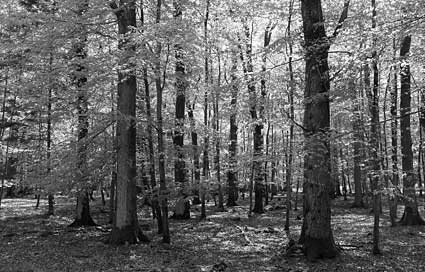
\includegraphics{./img/t1_original.png}
 \caption{Das Eingangsbild für alle Interpolationen in Task 1}
 \label{fig:t1_original}
\end{figure}

\clearpage


\section{Nearest Neighbor Interpolation}

Bei der Nearest Neighbor Interpolation wird der Pixelwert des Ausgabebildes durch den nächst gelegenen Pixel des Eingangsbildes gebildet. Das geschieht, indem einfach die Pixelkoordinaten auf den nächstgelegenen Integerwert gerundet werden. In Matlab wird dazu die Funktion \texttt{round} verwendet.

Der Algorithmus durchläuft alle Pixel des Ausgabebildes, berechnet die dazugehörigen exakten Pixelkoordinaten des Eingangsbildes, und rundet diese auf den nächsten Pixel.

\begin{equation}
 I_{out}(y_{out}, x_{out}) = I_{in}(round(y_{in}), round(x_{in}))
\end{equation}

Dadurch leidet die Qualität des Ergebnisses, weil eigentlich keine richtige Interpolation statt findet. Es wird nur der nächstgelegene Pixelwert verwendet, was unter anderem bei Kanten im Bild falsche Werte liefern kann. Durch die Einfachheit dieses Algorithmus ist er jedoch im Vergleich zu den anderen schnell.


\smallskip

Abbildung~\ref{fig:t1_nn} zeigt, das Ergebnis der Nearest Neighbor Interpolation. Man kann die falsch interpolierten Pixel gut erkennen, die durch die Wahl eines einzelnen Pixels entstehen (statt der Berechnung aus mehreren umliegenden Pixel). Die erreichte PSNR war 18.16dB.

\begin{figure}[htb]
 \centering
 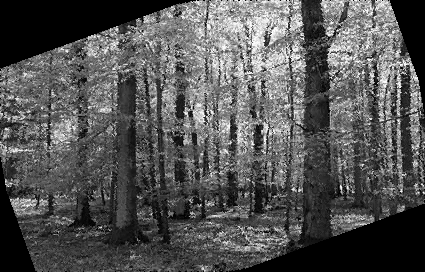
\includegraphics{./img/t1_nn.png}
 \caption{Das Ergebnis für Nearest Neighbor Interpolation in Task 1}
 \label{fig:t1_nn}
\end{figure}

\clearpage



\section{Bilineare Interpolation}
\label{t1_bl}

Bei der bilinearen Interpolation wird nicht mehr nur ein Pixel betrachtet, sondern die 4 naheliegendsten Pixel zu den berechneten Pixelkoordinaten (diese 4er-Nachbarschaft ist auf der händischen Berechnung zu Task 1 skizziert). Die umliegenden Pixel werden dabei mit der Distanz zu den berechneten Pixelkoordinaten gewichtet und aufsummiert. Die dazu verwendete Gewichtsfunktion $g(x)$ ist in der Aufgabenstellung angegeben, wobei x die Distanz zwischen exakten Pixelkoordinaten und dem tatsächlichen Pixel ist.

Der Algorithmus erstellt für das gesamte Bild zwei Matrizen, in denen die Pixelkoordinaten in x- bzw. y-Richtung gespeichert sind (Matlab-Funktion \texttt{meshgrid}). Jetzt wird das gesamte Bild durchlaufen, und für jeden Pixel die exakten Koordinaten berechnet. Aus diesen exakten Koordinaten und den Koordinatenmatrizen werden dann 2 Matrizen berechnet, die die Abstände aller Pixel zu den exakten Koordinaten enthalten. Diese Matrizen werden dann der Gewichtsfunktion \texttt{task1\_g} übergeben, welche daraus 2 Gewichtsmatrizen berechnet. Diese werden miteinander und mit dem Eingangsbild multipliziert, um alle gewichteten Pixel zu erhalten (die meisten dieser Pixel sind 0). Summiert man nun über die gesamte Matrix, so erhält man den interpolierten Wert für den aktuellen Pixel.
Diese Methode ist zwar einfach verständlich und übersichtlich, da aber die meisten Pixel 0 sind und dadurch bei der Berechnung wegfallen ist sie nicht effizient und hat eine lange Laufzeit. Sie beinhaltet aber bereits auch schon die Behandlung der außenliegenden Pixel, die dadurch einfach 0 gewertet werden, wodurch eine spezielle Randbehandlung überflüssig ist. Außerdem kann sie auch für die bikubische Interpolation (und auch andere Interpolationen) verwendet werden, wenn man einfach die Gewichtsfunktion \texttt{task1\_g} durch eine andere ersetzt.


\smallskip

Abbildung~\ref{fig:t1_bl} zeigt das Ergebnis der bilinearen Interpolation. Man erkennt, dass die Kanten im Bild nun viel glätter wirken, da die Ausgabepixel immer aus den 4 umliegenden Pixel berechnet werden. Allerdings entsteht durch diese Berechnung auch eine geringe Unschärfe gegenüber dem Originalbild. Durch die zusätzlichen Berechnungen ist die Laufzeit wesentlich länger als bei der Nearest Neighbor Interpolation. Die erreichte PSNR war 20.14dB, und damit höher als bei der Nearest Neighbor Interpolation. Das liegt an der genaueren Berechnung des Pixelwertes aus den umliegenden Pixel, anstatt einfach nur den nächsten Pixel zu verwenden.

\begin{figure}[htb]
 \centering
 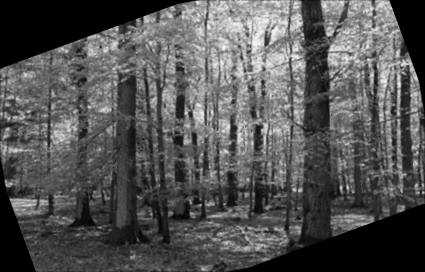
\includegraphics{./img/t1_bl.png}
 \caption{Das Ergebnis für bilineare Interpolation in Task 1}
 \label{fig:t1_bl}
\end{figure}

\clearpage



\section{Bikubische Interpolation}

Ähnlich der bilinearen Interpolation berechnet die bikubische Interpolation den Wert eine Pixels aus den den exakten Pixelkoordinaten umliegenden Pixelwerten. Anders als bei der bilinearen Interpolation werden hier jedoch nicht nur die 4 umliegenden Pixel, sondern 16 umliegende Pixel betrachtet. Diese werden dann mit einem Polynom gewichtet, dessen Koeffizienten variiert werden können um das Ergebnis zu beeinflussen. Bei schlechten Koeffizienten kann es bei der bikubischen Interpolation jedoch zu Ringing-Effekten (sichtbare ``Schwingungen'') kommen. Bei den hier verwendeten Koeffizienten entsteht jedoch ein schärfer wirkendes Bild.

Der Algorithmus ist gleich implementiert wie die bilineare Interpolation (siehe Abschnitt~\ref{t1_bl}). Der einzige Unterschied ist die Verwendung einer anderen Gewichtsfunktion \texttt{task1\_h}, welche nicht nach der Entfernung zu den exakten Pixelkoordinaten gewichtet, sondern je nach Entfernung ein Polynom berechnet. So werden mehrere Werte in der Gewichtsmatrix (die 16-er Nachbarschaft) ungleich 0 und für die Berechnung des Pixels verwendet. Da auch hier wieder viele Pixel in den Gewichtsmatrizen 0 sind, ist die Variante auch ineffizient (aber einfach) implementiert.

\smallskip

Abbildung~\ref{fig:t1_bc} zeigt das Ergebnis der bikubischen Interpolation. Im Vergleich zur bilinearen Interpolation ist das Ergebnis noch besser, die Unschärfe hat abgenommen. Durch das eingeführte Polynom als Gewichtsfunktion wirkt das Ausgabebild nochmals besser als bei der bilinearen Interpolation. Gleich wie bei der bilinearen Interpolation ist die Laufzeit auch wesentlich länger als bei der Nearest Neighbor Interpolation.

Die erreichte PSN war 24.11dB, also noch einmal wesentlich höher als bei der bilinearen Interpolation. Das liegt daran, dass der betreffende Pixel durch die Berechnung über das Polynom noch genauer bestimmt werden kann und so die Abweichungen auch nach mehreren Rotationen immer noch gering sind. Optisch sieht das Ergebnis der bikubischen Interpolation besser aus, es wirkt schärfer als das Ergebnis der bilinearen Interpolation.

\begin{figure}[htb]
 \centering
 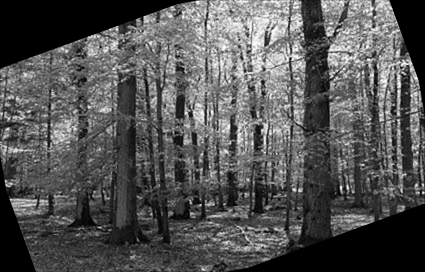
\includegraphics{./img/t1_bc.png}
 \caption{Das Ergebnis für bikubische Interpolation in Task 1}
 \label{fig:t1_bc}
\end{figure}

\clearpage



\chapter{Task 2: Denoising}

Ziel von Task 2 war es, vorgegebene Bilder zu entrauschen. Dabei waren diese entweder mit weißem Rauschen (AWGN), Salt and Pepper Noise oder Specle Noise überlagert. Dazu wurden 3 unterschiedliche Filter implementiert:

\begin{itemize}
 \item \emph{Mittelwertfilter:} bildet den Mittelwert über einen bestimmten Bildbereich. Ein Filterkernel wird berechnet, und per Faltung angewandt. Es handelt sich um einen linearen Filter.
 
 \item \emph{Gaussfilter:} bildet ähnlich wie der Mittelwertfilter einen Mittelwert über einen bestimmten Bildbereich, jedoch gewichtet mit einer Gaussfunkion mit unterschiedlichem $\sigma$.
 
 \item \emph{Medianfilter:} bildet den Median in einem bestimmten Bildbereich (ordnet die Pixelwerte aufsteigend und wählt den in dieser Sortierung mittigen Pixelwert). Dieser Filter ist nichtlinear und kann deswegen nicht durch Faltung berechnet werden.
\end{itemize}

Diese 3 Filter wurden dann mit unterschiedlichen Parametern auf die verrauschten Eingangsbilder angewandt, und in Hinsicht auf die PSNR mit den Originalbildern untersucht. Im folgenden Abschnitt werden die verwendeten Filter kurz beschrieben und einige Ergebnisse zur Veranschaulichung dargestellt.


Abbildungen~\ref{fig:t2_b}, \ref{fig:t2_e} und \ref{fig:t2_g} zeigen die verrauschten Ausgangsbilder und deren PSNR.

\begin{figure}[htb]
 \centering
 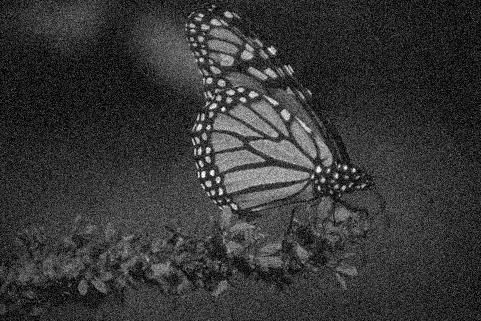
\includegraphics[width=0.7\textwidth]{../images/noise_butterfly.jpg}
 \caption{Verrauschtes Testbild ``Butterfly'' für Task 2, PSNR = 22.56dB}
 \label{fig:t2_b}
\end{figure}

\begin{figure}[htb]
 \centering
 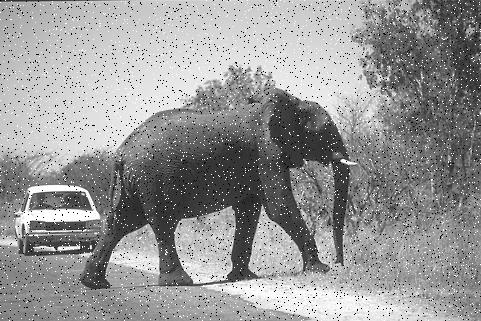
\includegraphics[width=0.7\textwidth]{../images/noise_elephant.jpg}
 \caption{Verrauschtes Testbild ``Elephant'' für Task 2, PSNR = 17.92dB}
 \label{fig:t2_e}
\end{figure}

\begin{figure}[htb]
 \centering
 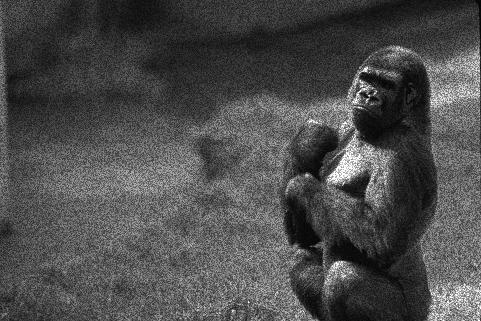
\includegraphics[width=0.7\textwidth]{../images/noise_gorilla.jpg}
 \caption{Verrauschtes Testbild ``Gorilla'' für Task 2, PSNR = 22.1dB}
 \label{fig:t2_g}
\end{figure}

\clearpage



\section{Mittelwertfilter}

Der Mittelwertfilter bildet den Mittelwert über einen bestimmten Bildbereich, der von der Kernelgröße bestimmt wird. Dazu wird ein Filterkernel generiert, der für alle Elemente den gleichen Wert hat. Dieser Wert muss über den gesamten Kernel die Summe 1 ergeben. Je nach Größe des Kernels wird ein unterschiedlich großer Bildbereich gemittelt. Faltet man das Bild dann mit dem Kernel, wird für jeden Pixel der Mittelwert der umliegenden Pixel berechnet. Dadurch wird das Bild geglättet, durch die unendlich steilen Flanken am Rand des Kernels kann es aber zu Ringing-Effekten kommen.

\smallskip

Im Folgenden werden die Ergebnisse der Filterung mit dem Mittelwertfilter dargestellt. Wenn nicht anders angegeben, wurde die Filtergröße so gewählt, dass sich die höchste PSNR ergibt.

Abbildung~\ref{fig:t2_b_a3} zeigt das Ergebnis des Mittelwertfilters beim Testbild ``Butterfly''. Die höchste PSNR mit 29.82dB wurde bei einer Filtergröße von $3 \cdot 3$ Pixel erreicht. Dieses Ergebnis ist bereits recht gut. Erhöht man jedoch die Größe des Filterkernels z.B. auf $11 \cdot 11$ Pixel, so kann man bereits deutliche Ringing-Effekte erkennen (siehe Abbildung~\ref{fig:t2_b_a11_ring}).

Abbildung~\ref{fig:t2_e_a3} zeigt das Ergebnis beim Testbild ``Elephant'' (Größe $3 \cdot 3$). Dieses Bild ist mit Salt and Pepper Noise überlagert, dieses fließt jedoch direkt in die Berechnung des Mittelwerts ein. Auch nach der Filterung ist die Störung noch deutlich sichtbar, die PSNR ist mit 24.56dB deswegen entsprechend niedrig. Eine Vergrößerung des Filterkernels auf z.B. $7 \cdot 7$ bringt auch keine großen Erfolge, die Störung ist immer noch sichtbar (Abbildung~\ref{fig:t2_e_a7_}).

Abbildung~\ref{fig:t2_g_a5} zeigt das Ergebnis beim Testbild ``Gorilla'' (Größe $5 \cdot 5$). Auch hier kann eine relativ hohe PSNR von 30.18dB erreicht werden, natürlich kommt es zum Schärfeverlust.

\smallskip

\begin{figure}[htb]
 \centering
 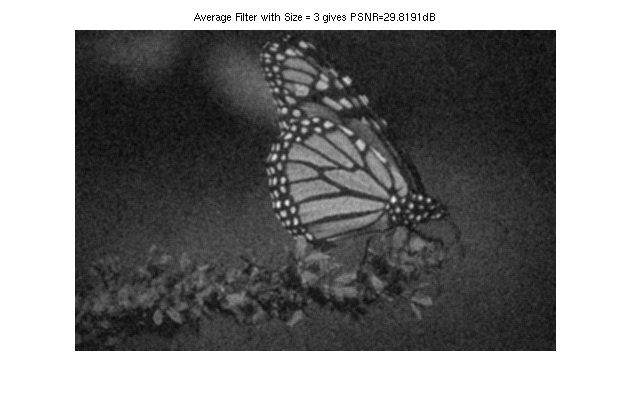
\includegraphics[width=0.7\textwidth]{../images_out/t2_b_a3.png}
 \caption{Testbild ``Butterfly'', mittelwertgefiltert mit $N=3$}
 \label{fig:t2_b_a3}
\end{figure}

\begin{figure}[htb]
 \centering
 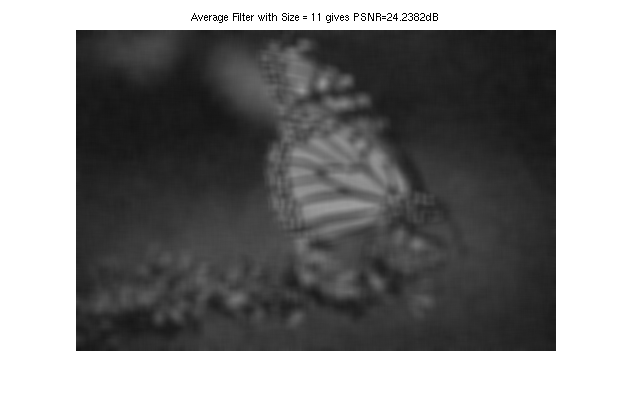
\includegraphics[width=0.7\textwidth]{../images_out/t2_b_a11_ring.png}
 \caption{Testbild ``Butterfly'', mittelwertgefiltert mit $N=11$, Ringing-Effekt sichtbar}
 \label{fig:t2_b_a11_ring}
\end{figure}

\begin{figure}[htb]
 \centering
 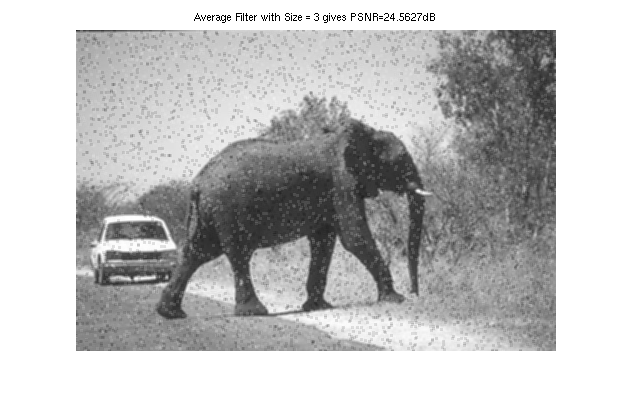
\includegraphics[width=0.7\textwidth]{../images_out/t2_e_a3.png}
 \caption{Testbild ``Elephant'', mittelwertgefiltert mit $N=3$, Salt and Pepper Noise sichtbar}
 \label{fig:t2_e_a3}
\end{figure}

\begin{figure}[htb]
 \centering
 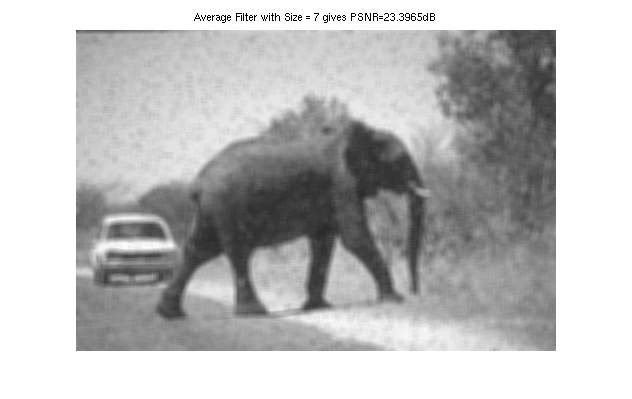
\includegraphics[width=0.7\textwidth]{../images_out/t2_e_a7_.png}
 \caption{Testbild ``Elephant'', mittelwertgefiltert mit $N=7$, Salt and Pepper Noise noch immer sichtbar}
 \label{fig:t2_e_a7_}
\end{figure}

\begin{figure}[htb]
 \centering
 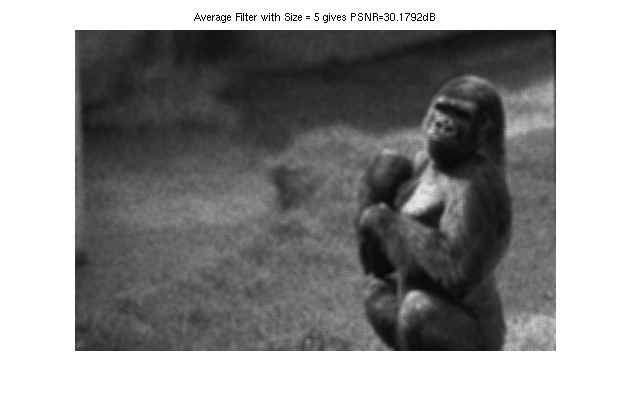
\includegraphics[width=0.7\textwidth]{../images_out/t2_g_a5.png}
 \caption{Testbild ``Gorilla'', mittelwertgefiltert mit $N=5$}
 \label{fig:t2_g_a5}
\end{figure}

\clearpage


\section{Gaussfilter}

Der Gaussfilter verwendet eine Gaussfunktion, um einen gewichteten Mittelwert aus den umliegenden Pixel zu berechnen. Dadurch wird der mittlere (betroffene) Pixel stärker gewichtet wie die umliegenden, es erfolgt eine sanftere Glättung als beim Mittelwertfilter. Durch die weichen Übergänge wird außerdem der Ringing-Effekt verhindert. Der Gaussfilter wird für ein bestimmtes $\sigma$ generiert (die Formel für die Berechnung ist in der Aufgabenstellung angegeben), die Größe des Kernels wird aus dem verwendeten $\sigma$ berechnet.

\smallskip

Im Folgenden werden die Ergebnisse der Filterung mit dem Gaussfilter dargestellt. Wenn nicht anders angegeben, wurde der Parameter $\sigma$ so gewählt, dass sich die höchste PSNR ergibt.

Abbildung~\ref{fig:t2_b_g091} zeigt das Ergebnis des Gaussfilters beim Testbild ``Butterfly''. Die höchste PSNR mit 30.22dB wurde bei $\sigma = 0.91$ erreicht. Dieses Ergebnis ist besser als beim Mittelwertfilter. Optisch ist jedoch nicht viel Unterschied zu erkennen. Beim Gaussfilter kommt es auch bei höherem $\sigma$ zu keinen Ringing-Artefakten, das Bild wird lediglich unschärfer (siehe Abbildung~\ref{fig:t2_b_g3_smooth}, $\sigma = 3$).

Abbildung~\ref{fig:t2_e_g101} zeigt das Ergebnis beim Testbild ``Elephant'' ($\sigma = 1.01$). Wie beim Mittelwertfilter kann das Salt and Pepper Noise durch den Gaussfilter nicht entfernt werden. Die PSNR beträgt maximal 25.21dB.

Abbildung~\ref{fig:t2_g_g119} zeigt das Ergebnis beim Testbild ``Gorilla'' ($\sigma = 1.19$). Die erreichte PSNR liegt bei 31.01dB, also noch höher als beim Mittelwertfilter.

\smallskip

\begin{figure}[htb]
 \centering
 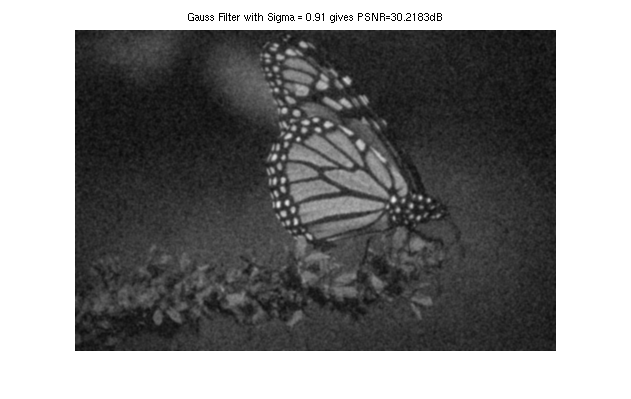
\includegraphics[width=0.7\textwidth]{../images_out/t2_b_g091.png}
 \caption{Testbild ``Butterfly'', Gauss-gefiltert mit $\sigma=0.91$}
 \label{fig:t2_b_g091}
\end{figure}

\begin{figure}[htb]
 \centering
 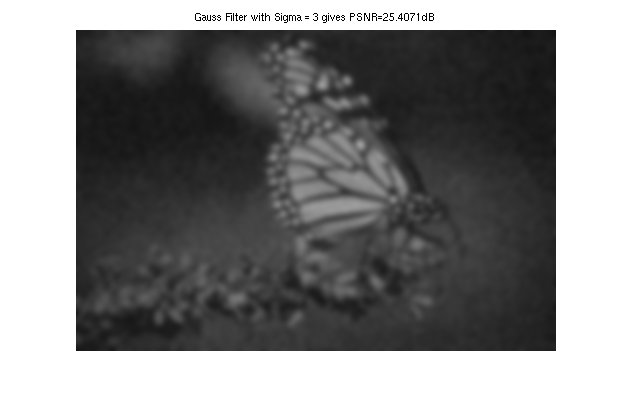
\includegraphics[width=0.7\textwidth]{../images_out/t2_b_g3_smooth.png}
 \caption{Testbild ``Butterfly'', Gauss-gefiltert mit $\sigma=3$, unscharf}
 \label{fig:t2_b_g3_smooth}
\end{figure}

\begin{figure}[htb]
 \centering
 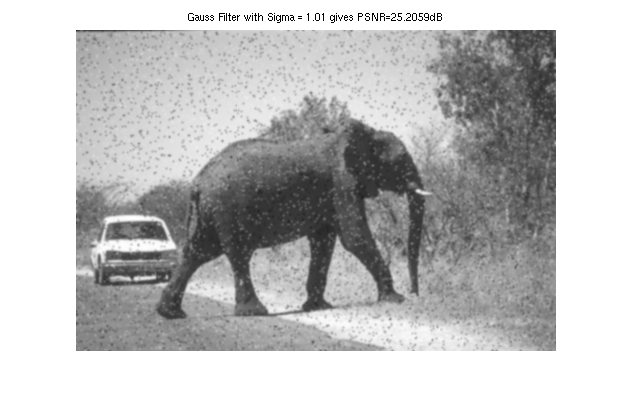
\includegraphics[width=0.7\textwidth]{../images_out/t2_e_g101.png}
 \caption{Testbild ``Elephant'', Gauss-gefiltert mit $\sigma=1.01$}
 \label{fig:t2_e_g101}
\end{figure}

\begin{figure}[htb]
 \centering
 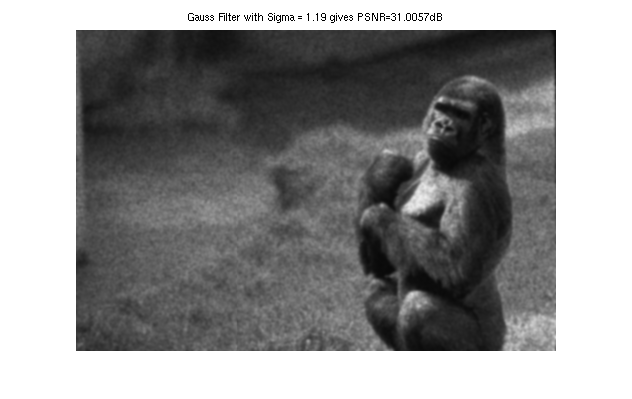
\includegraphics[width=0.7\textwidth]{../images_out/t2_g_g119.png}
 \caption{Testbild ``Gorilla'', Gauss-gefiltert mit $\sigma=1.19$}
 \label{fig:t2_g_g119}
\end{figure}

\smallskip

Außer beim Salt and Pepper Noise erreicht der Gaussfilter die besten Ergebnisse aller hier aufgeführten Filter.

\clearpage



\paragraph{Laufzeit}

Zusätzlich sollte für den Gaussfilter die Laufzeit untersucht und mit der eingebauten Funktion \texttt{imfilter} verglichen werden. Dazu wurde ein großer Filterkernel generiert, um die Berechnung möglichst lange dauern zu lassen. Mit den Befehlen \texttt{tic} und \texttt{toc} wurden dann die Laufzeiten der beiden Implementierungen bestimmt:

\smallskip

\texttt{Homebrew Gauss filter execution time: 0.83439s}
 
\texttt{Matlab imfilter Gauss filter execution time: 0.02085s}

\smallskip

Der große Unterschied liegt an der hochoptimierten Implementierung von \texttt{imfilter} im Vergleich zur primitiven Implementierung für diese Aufgabenstellung. Es gäbe mehrere Möglichkeiten, die Leistung zu verbessern, zum Beispiel:

\begin{itemize}
 \item Aufteilen des 2-dimensionalen Filterkernels in zwei 1-dimensionale Filterkerne und hintereinanderfolgende Faltung des Bildes mit den 2 Filterkerneln in x- und y-Richtung. Die Anzahl der Berechnungen nimmt dann drastisch ab
 
 \item Statt einer aufwändigen Faltung im Bildbereich kann eine einfache Matrizenmultiplikation im Frequenzbereich durchgeführt werden. Dazu werden das Bild und der Filterkernel Fourier-transformiert, miteinander multipliziert, und zurücktransformiert. Voraussetzung dafür ist jedoch eine schnelle Implementierung der Fouriertransformation (FFT).
\end{itemize}

\clearpage



\section{Medianfilter}

Der Medianfilter berechnet den Median über einen bestimmten Bildbereich, indem alle Pixel in der Umgebung (definiert durch die Größe des Filters) aufsteigend sortiert werden und der in dieser Reihenfolge mittige Wert verwendet. Es handelt sich also um einen nichtlinearen Filter, der nicht durch Faltung angewandt werden kann. Stattdessen wird das Originalbild mehrmals verschoben, so dass jeweils eine verschobene Matrix entsteht, deren betroffener Pixel an der gleichen Position ist wie der mittige Pixel in der Originalmatrix. Bei einer Filtergröße von $3 \cdot 3$ müssen also 8 Matrizen berechnet werden, die die verschobenen Bilder enthalten. Legt man diese Matrizen 3-dimensional übereinander, so kann die Matlab-Funktion \texttt{median} verwendet werden, um den Median für jeden Pixel auszurechnen (in der z-Dimension). Dadurch erhält man eine Matrix, die den Median für alle Pixel enthält. Diese Methode ist schnell, benötigt jedoch mehr Speicher als eine iterative Version. Der Vorteil des Medianfilters ist, dass Ausreißer ignoriert werden. Dadurch eignet sich der Medianfilter besonders bei Salt and Pepper Noise.

\smallskip

Im Folgenden werden die Ergebnisse der Filterung mit dem Medianfilter dargestellt. Wenn nicht anders angegeben, wurde Filtergröße so gewählt, dass sich die höchste PSNR ergibt.

Abbildung~\ref{fig:t2_b_m3} zeigt das Ergebnis des Medianfilters beim Testbild ``Butterfly''. Die höchste PSNR mit 28.74dB wurde bei der Größe $3 \cdot 3$ erreicht. Dieses Ergebnis ist das schlechteste der 3 Filter. Ein mittelwertbildender Filter funktioniert bei dieser Störung besser. Erhöht man die Größe des Medianfilters, zeichnen sich die Kanten im Bild mehr ab (siehe Abbildung~\ref{fig:t2_b_m11_}, Größe $11 \cdot 11$).

Abbildung~\ref{fig:t2_e_m3} zeigt das Ergebnis beim Testbild ``Elephant'' (Größe $3 \cdot 3$). Beim Salt and Pepper Noise kann der Medianfilter seine Stärken ausspielen, indem die weißen und schwarzen Pixel als Ausreißer ignoriert werden. Die PSNR beträgt 28.04dB und ist damit die höchste unter allen Filtern.

Abbildung~\ref{fig:t2_g_m5} zeigt das Ergebnis beim Testbild ``Gorilla'' (Größe $5 \cdot 5$). Die erreichte PSNR liegt bei 29.05dB, hier kann mit den anderen Filtern eine etwas höhere PSNR erreicht werden.

\smallskip

\begin{figure}[htb]
 \centering
 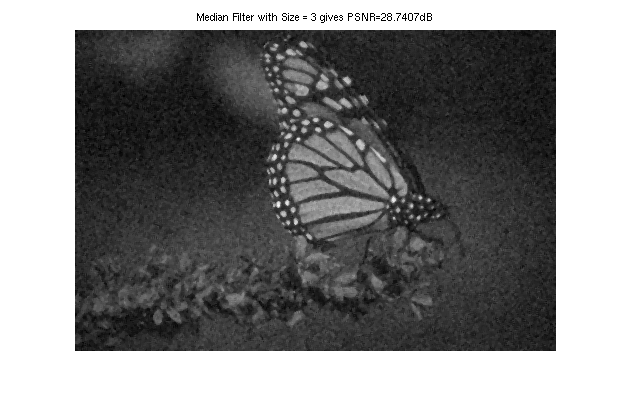
\includegraphics[width=0.7\textwidth]{../images_out/t2_b_m3.png}
 \caption{Testbild ``Butterfly'', mediangefiltert mit Größe $3 \cdot 3$}
 \label{fig:t2_b_m3}
\end{figure}

\begin{figure}[htb]
 \centering
 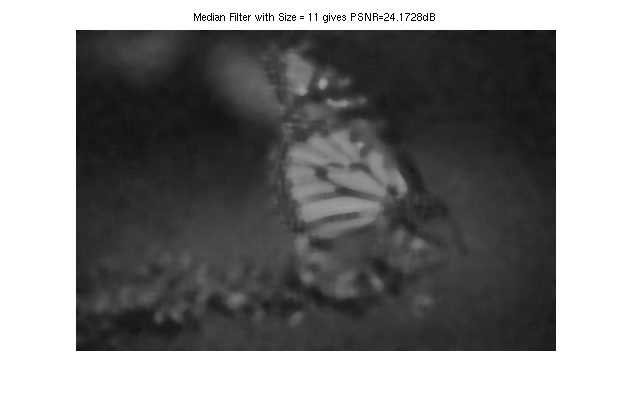
\includegraphics[width=0.7\textwidth]{../images_out/t2_b_m11_.png}
 \caption{Testbild ``Butterfly'', mediangefiltert mit Größe $11 \cdot 11$, Kanten zeichnen sich ab}
 \label{fig:t2_b_m11_}
\end{figure}

\begin{figure}[htb]
 \centering
 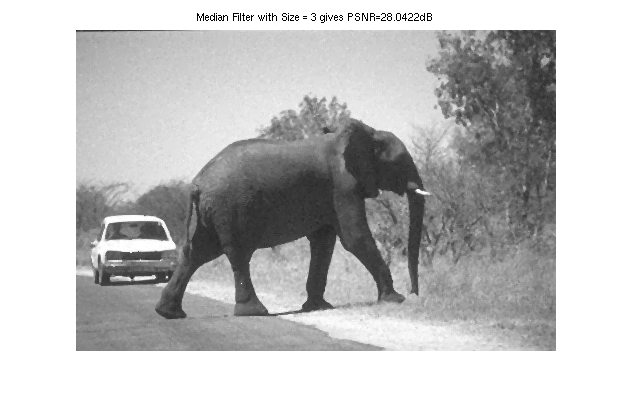
\includegraphics[width=0.7\textwidth]{../images_out/t2_e_m3.png}
 \caption{Testbild ``Elephant'', mediangefiltert mit Größe $3 \cdot 3$}
 \label{fig:t2_e_m3}
\end{figure}

\begin{figure}[htb]
 \centering
 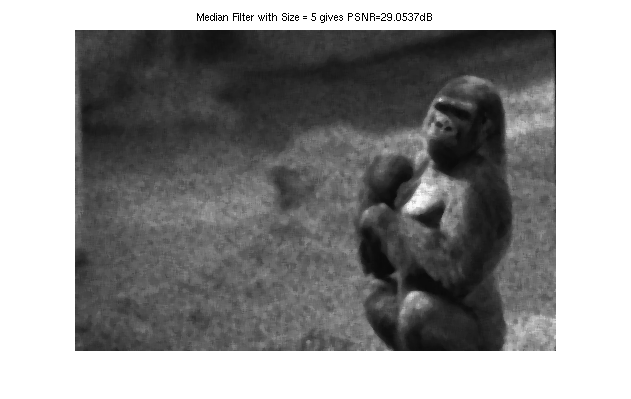
\includegraphics[width=0.7\textwidth]{../images_out/t2_g_m5.png}
 \caption{Testbild ``Gorilla'', mediangefiltert mit Größe $5 \cdot 5$}
 \label{fig:t2_g_m5}
\end{figure}

\clearpage



\chapter{Bonus Task: Denoising}

In diesem Task wurde folgendes Bild mit Störung angegeben:

\begin{figure}[h!]
 \centering
 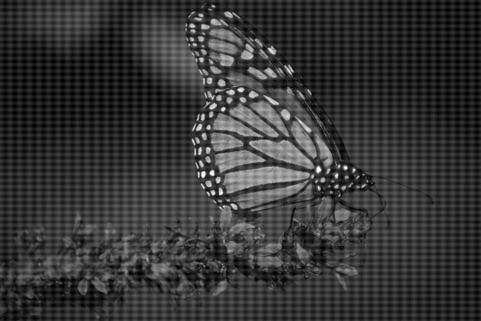
\includegraphics[width=0.7\textwidth]{../images/bonus.png}
 \caption{Gestörtes Bild für den Bonustask}
 \label{fig:b_original}
\end{figure}

Man erkennt die wellenförmigen Streifen in horizontaler und vertikaler Richtung. Betrachtet man das Bild im Frequenzbereich, sieht man den Ursprung dieser Störung:

\begin{figure}[h!]
 \centering
 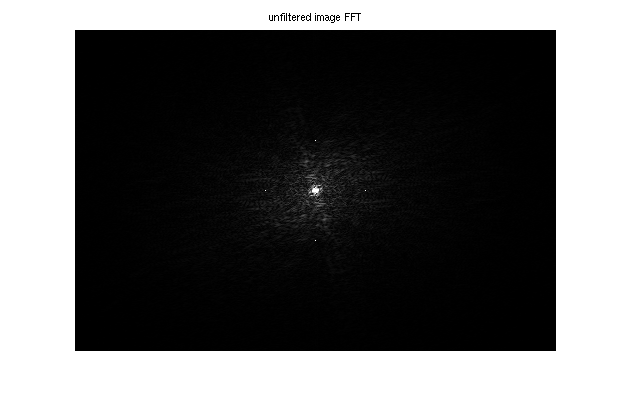
\includegraphics[width=0.7\textwidth]{../images_out/b_unfiltered_fft.png}
 \caption{FFT des gestörten Bildes für den Bonustask}
 \label{fig:b_unfiltered_fft}
\end{figure}

Der helle Bereich im Zentrum ist der größte Anteil der Bildinformation. Auffallend sind die 4 hellen Punkte im gleichen Abstand um das Zentrum. Diese einzelnen Punkte entsprechen einer Überlagerung mit einem sinusförmigen Signal in horizontaler und vertikaler Richtung (der Abstand zum Zentrum im FFT-Bild gibt die Ortsfrequenz des Störsignals an). Dieses Störsignal kann aus verschiedenen Gründen in das Bild kommen, beispielsweise:

\begin{itemize}
 \item das Abtasttheorem wurde nicht eingehalten, bei der Störung handelt es sich um Aliasing
 \item bei einer analogen Übertragung des Nutzsignals wurden diese Sinusschwingungen mit empfangen
\end{itemize}

Um die Streifen zu entfernen, müssen die Störfrequenzen entfernt werden. Dies geht im Frequenzbereich recht einfach. Die 4 hellen Punkte werden aus der FFT-Darstellung entfernt, und dieses Bild wird dann wieder in den Ortsbereich zurücktransformiert. Die Störung sollte dann entfernt sein.

Im einfachsten Fall können die entsprechenden Pixel in der FFT-Darstellung auf 0 gesetzt. In der Praxis wären diese Störungen jedoch wahrscheinlich keine einzelnen Pixel, sondern eine Anhäufung von Pixeln. Außerdem kommt es durch die extreme Flankensteilheit beim Entfernen von nur einem gewissen Pixel leicht zu Ringing-Effekten, deswegen sollten die Störungen mit einem Gaussfilter mit geringem $\sigma$ entfernt werden.

Zum Entfernen der Störung wurden nun folgende Schritte durchgeführt:

\begin{itemize}
 \item Transformation des Bildes in den Frequenzbereich
 \item Finden der exakten Positionen der Störungen:
	\begin{itemize}
	 \item Hochpassfiltern des Bildes, um die Hauptinformation in der Mitte der FFT-Darstellung zu entfernen (ein unnormierter Gausskernel mit großem $\sigma$ entfernt die Information komplett)
	 \item Finden der Maxima in der hochpassgefilterten FFT-Darstellung ergibt die 4 Punkte
	\end{itemize}
 \item Generieren eines weichen Notch-Filters zum Entfernen der 4 Störungen:
  \begin{itemize}
   \item Erzeugen einer Matrix mit Wert 1 an der exakten Position der Störungen, ansonsten mit Wert 0
   \item Falten dieser Matrix mit einem invertierten, unnormierten Gausskernel mit geringem $\sigma$
   \item es entsteht eine Matrix mit auf den Wert 0 abfallenden Gaussglocken genau an den Positionen der Störungen
  \end{itemize}
 \item FFT-Darstellung mit dem entstandenen Notch-Filter multiplizieren, die Störungen werden so entfernt
 \item Rücktransformation in den Bildbereich
\end{itemize}

Abbildung~\ref{fig:b_notch} zeigt den Notch-Filter im Frequenzbereich. Multipliziert man diesen mit der FFT-Darstellung des gestörten Bildes (Abbildung~\ref{fig:b_unfiltered_fft}) entsteht ein Frequenzspektrum ohne diese Störungen (siehe Abbildung~\ref{fig:b_filtered_fft}). Wird dieses nun in den Bildbereich rücktransformiert, entsteht ein ungestörtes Bild (siehe Abbildung~\ref{fig:b_filtered}). Die PSNR ergibt sich zu 56.62dB (gestörtes Bild: PSNR=26.03dB).

\begin{figure}[htb]
 \centering
 \includegraphics[width=0.7\textwidth]{../images_out/b_notch.png}
 \caption{Verwendeter Notch-Filter im Frequenzbereich}
 \label{fig:b_notch}
\end{figure}

\begin{figure}[htb]
 \centering
 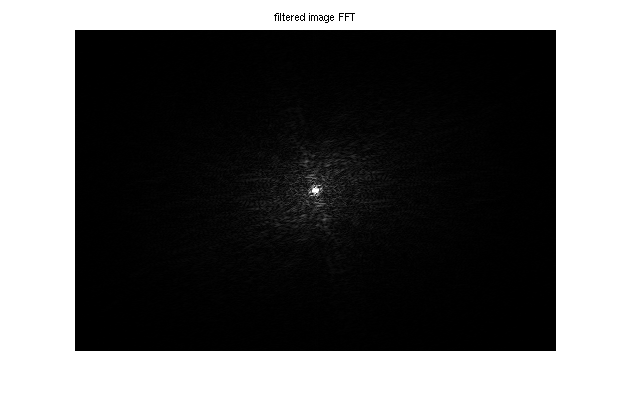
\includegraphics[width=0.7\textwidth]{../images_out/b_filtered_fft.png}
 \caption{FFT des entstörten Bildes für den Bonustask}
 \label{fig:b_filtered_fft}
\end{figure}

\begin{figure}[htb]
 \centering
 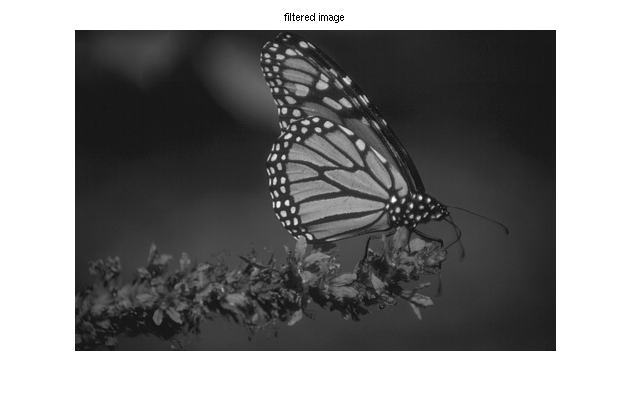
\includegraphics[width=0.7\textwidth]{../images_out/b_filtered.png}
 \caption{Entstörtes Bild für den Bonustask}
 \label{fig:b_filtered}
\end{figure}

\clearpage




\chapter{Task 3: Canny Edge Detector}

In Task 3 sollte ein Canny Edge Detector verwendet werden. In den folgenden Kapiteln werden die einzelnen Schritte erklärt und alle Zwischenschritte dargestellt.

Als Eingangsbild wurde das Testbild ``Elephant'' verwendet (siehe Abbildung~\ref{fig:t2_e}).


\section{Gaussfiltern}

Der erste Schritt ist die Gaussfilterung. Da Störungen (Noise) den Kantendetektor anschlagen lassen können, darf auf diesen Schritt nicht verzichtet werden. Dabei handelt es sich um eine einfache Faltung mit einem Gausskernel. Dazu wurden die Matlab-Funktionen \texttt{imfilter} und \texttt{fspecial} verwendet.

Je nach gewünschter Genauigkeit beim Erkennen von Kanten kann der Parameter $\sigma$ gewählt werden. Sollen nur Kanten in groben Strukturen erkannt werden, wählt man $\sigma$ groß, sollen auch feine Strukturen erkannt werden, wählt man $\sigma$ klein. Für dieses Beispiel wurde $\sigma = 0.8$ gewählt.


\section{Gradienten berechnen}

In diesem Schritt werden die Gradienten des Bildes (die Ableitungen) in x- und y-Richtung berechnet ($G_x$ und $G_y$). Dazu wurde ein Sobel-Kernel in x- und y-Richtung verwendet (Matlab-Befehl \texttt{fspecial}), und das Bild mit diesen Kerneln gefaltet.

Zur Berechnung von Norm (Magnitude) und Angle wurden folgende Zusammenhänge verwendet:

\begin{equation}
 \left|G\right| = \sqrt{G_x^2 + G_y^2}
\end{equation}

\begin{equation}
 \varphi = atan \left( \frac{G_y}{G_x} \right)
\end{equation}

Abbildungen~\ref{fig:t3_sobel_x} und \ref{fig:t3_sobel_y} zeigen die berechneten Gradienten, Abbildung~\ref{fig:t3_magnitude} zeigt die berechnete Norm. Man kann bereits die starken Kanten recht gut erkennen.

\smallskip

\begin{figure}[htb]
 \centering
 \includegraphics[width=0.7\textwidth]{../images_out/t3_sobel_x.png}
 \caption{Ergebnis des Sobel-Operators in x-Richtung}
 \label{fig:t3_sobel_x}
\end{figure}

\begin{figure}[htb]
 \centering
 \includegraphics[width=0.7\textwidth]{../images_out/t3_sobel_y.png}
 \caption{Ergebnis des Sobel-Operators in y-Richtung}
 \label{fig:t3_sobel_y}
\end{figure}

\begin{figure}[htb]
 \centering
 \includegraphics[width=0.7\textwidth]{../images_out/t3_magnitude.png}
 \caption{Berechnete Magnitude der Gradienten}
 \label{fig:t3_magnitude}
\end{figure}

\clearpage

\section{Non-Maximum Suppression}

Nach diesem Schritt bleiben nur die lokalen Maxima übrig. Bei Kanten, die aus mehreren nebeneinander liegenden Pixelreihen bestehen, bleibt nur die tatsächliche Kante über, also die Pixelreihe mit der höchsten Amplitude.

Dazu wird überprüft, ob die Pixel, die normal auf die Kantenrichtung stehen, größere Werte haben als das Kantenpixel. Falls ja, handelt es sich beim aktuellen Kantenpixel nicht um das lokale Maximum, und es wird aus dem Bild entfernt. Dazu wird die Funktion \texttt{histc} verwendet, um alle Kantenrichtungen auf 4 prinzipielle Richtungen zu runden:

\begin{itemize}
 \item horizontale Kanten (0°)
 \item vertikale Kanten (-90°/90°)
 \item diagonale, steigende Kanten (45°)
 \item diagonale, fallende Kanten (-45°)
\end{itemize}

Je nach prinzipieller Kantenrichtung wird jetzt überprüft, ob die normal auf der Kante stehenden Pixel größere Werte haben, als das aktuelle Kantenpixel. Falls ja, wird das aktuelle Kantenpixel 0 gesetzt. Diese Berechnung wird beschleunigt, indem 8 Matrizen berechnet werden, in denen das Bild um jeweils einen Pixel in alle Richtungen verschoben ist. Um herauszufinden, ob das Kantenpixel kleiner ist als die Umliegenden Pixel, müssen nur die entsprechenden verschobenen Bilder vom Originalbild subtrahiert werden. Ist das Ergebnis negativ, ist das aktuelle Kantenpixel kein Maximum und kann entfernt werden.

Abbildung~\ref{fig:t3_nonmax} zeigt das Ergebnis der Non-Maximum-Suppression. Man erkennt, das wirklich nur mehr die stärksten Kanten übrig sind, und nicht mehr viele abgestufte Kanten nebeneinander liegen.

Zum besseren Verständnis der Zuordnung der Kantenrichtung wurde das Ergebnis der Non-Maximum Suppression mit einem Threshold von 0.7 gefiltert, und die entstehenden Kanten nach ihrer zugeordneten Orientierung eingefärbt. Das Ergebnis ist in Abbildung~\ref{fig:t3_nonmax_angles} dargestellt.

\smallskip

\begin{figure}[htb]
 \centering
 \includegraphics[width=0.7\textwidth]{../images_out/t3_nonmax.png}
 \caption{Magnitude nach der Non-Maximum Suppression}
 \label{fig:t3_nonmax}
\end{figure}

\begin{figure}[htb]
 \centering
 \includegraphics[width=0.7\textwidth]{../images_out/t3_nonmax_angles.png}
 \caption{Eingefärbte Kanten entsprechend der erkannten Orientierung}
 \label{fig:t3_nonmax_angles}
\end{figure}

\clearpage



\section{Double Thresholding}

Nach der Non-Maximum Suppression werden nun die gefundenen Kanten mit 2 Thresholds beaufschlagt. Dazu wurden in diesem Beispiel die Thresholds 0.4 und 0.8 gewählt. Alle Pixel, die einen Wert kleiner als den unteren Threshold haben, werden sofort als Nicht-Kanten bewertet und aus dem Kantenbild entfernt. Alle Pixel mit Werten zwischen den Thresholds werden als \emph{weak edges} gewertet, und mit dem Kantenwert 0.6 initialisiert. Alle Pixel, die einen Kantenwert über dem oberen Threshold haben, werden als \emph{strong edges} bewertet und mit dem Kantenwert 1 initialisiert (der Maximalwert).

Mit dem Variieren der Thresholds kann bestimmt werden, welche Kantenstärke ausreicht, um eine Kante zu erkennen.

Abbildung~\ref{fig:t3_threshold} zeigt das Ergebnis nach diesem Schritt. Man erkennt die \emph{weak edges} (grau) und die \emph{strong edges} (weiß).

\smallskip

\begin{figure}[htb]
 \centering
 \includegraphics[width=0.7\textwidth]{../images_out/t3_threshold.png}
 \caption{Kantenstärke nach dem Double Thresholding}
 \label{fig:t3_threshold}
\end{figure}

\clearpage



\section{Hysteresis}

Nach dem Thresholding muss nun ein Binärbild mit den erkannten Kanten erstellt werden. Zuerst werden alle bereits erkannten \emph{strong edges} in das Binärbild übernommen. Dann werden die 8er-Nachbarschaften aller \emph{weak edges} untersucht. Befindet sich in der Nachbarschaft eine \emph{strong edge}, so wird die weak edge ebenfalls zur strong edge erklärt und in das Binärbild eingefügt. Dieser Schritt wird so lange wiederholt, bis keine neue strong edge mehr hinzugekommen ist.

Um die Nachbarschaft zu untersuchen, wird das aktuelle Binärbild mit den strong edges wieder in jede Richtung um einen Pixel verschoben und mit einem logischen \emph{oder}-Operator verknüpft. Befindet sich in mindestens einem Pixel der 8er-Nachbarschaft eine strong edge, ergibt diese Verknüpfung ein logisches \emph{true}. Ist an dem entsprechenden Pixel nun eine weak edge, so wird diese zur strong edge erklärt.

Wird dieser Schritt immer wieder wiederholt, breiten sich die strong edges so lange aus, bis keine weak edges mehr vorhanden sind, die die Bedingung erfüllen. Die Iteration terminiert dann, und das aktuelle Binärbild mit den strong edges wird zum Ergebnis-Kantenbild erklärt. Abbildung~\ref{fig:t3_result} zeigt das Ergebnis für das angegebene Beispiel.

\smallskip

\begin{figure}[htb]
 \centering
 \includegraphics[width=0.7\textwidth]{../images_out/t3_result.png}
 \caption{Endergebnis nach der Hysteresebildung}
 \label{fig:t3_result}
\end{figure}

\clearpage



% **************************************************************************************************
% **************************************************************************************************

%\appendix
%\bibliographystyle{/.base/ieeetran}
%\bibliography{_bibliography}

% place all floats and create label on last page
\FloatBarrier\label{end-of-document}
\end{document}

